\section{Module Introduction}

%\begin{frame}{Introduction to SM-2302}
%	\tableofcontents
%\end{frame}

\subsection{Module content}
\begin{frame}{Welcome to SM-2302}
Mathematical software is what bridges higher mathematics to real world applications. 
On completing this module, students should be able to use \txt{MATLAB} and \txt{R} to effectively 
implement mathematical solutions to real world problems. 
They should also be able to produce publication-quality mathematical documents using \LaTeX. 
This module provides the computing skills required for an applied mathematics final year project.

\par\bigskip 
{\bfseries Module content}
\par\smallskip

\begin{enumerate}
	\item Introduction to the \txt{MATLAB} and \txt{R} languages.
	\item Programming using \txt{MATLAB} and \txt{R}.
	\item Preparing documents using \LaTeX.
	\item Version control using Git and GitHub.
\end{enumerate}
\end{frame}


\begin{frame}
\begin{exampleblock}{Assessment:~\textbf{100\% coursework}}
\begin{enumerate}
	\item Four online quizzes (20\%)
	\item Two mini individual assignments (20\%)
	\item Two mini group assisgnments (30\%)
	\item One project assignment with written report (30\%)
\end{enumerate}
\end{exampleblock}

\par\bigskip 
{\bfseries Weekly contact hours}
\par\smallskip
\begin{itemize}
	\item \underline{Lectures}:~ 2 hours in computer lab on Thursdays 7:50 AM
	\item \underline{Tutorials}:~ 2 hours practice lab on Saturdays 2:10 PM
\end{itemize} 
See full schedule in the \href{https://sm2302.github.io/sm2302-syllabus.pdf}{SM-2302 Syllabus document}.
\end{frame}

\subsection{Getting started with \txt{MATLAB}}
\begin{frame}{\txt{MATLAB}}
\begin{itemize}
	\item \txt{MATLAB} is a high-level language and interactive environment for numerical computation,
	visualization and programming.
	\begin{itemize}
		\item Analyze data
		\item Develop algorithms
		\item Create models and applications
	\end{itemize}
	\item We will reinforce some calculus concepts and its applications using \txt{MATLAB}, such as
	\begin{itemize}
		\item Numerical differentiation
		\item Numerical Integration
		\item Root-finding methods
	\end{itemize}
\end{itemize}
\end{frame}

\begin{frame}{Software}
\txt{MATLAB} is installed in the campus computer labs. 
However, if you wish to work from home or on your laptop, you can either
\begin{enumerate}
	\item use \txt{MATLAB} Online on your web browser; or
	\item install \txt{MATLAB} on your personal computer. 
\end{enumerate}

\begin{alertblock}{MATLAB Campus-wide suite}
To install or use \txt{MATLAB} on your web browser, you need to create a Mathworks
account using your UBD e-mail. You can access the UBD campus-wide suite using your mathworks account.\\
Please refer to the \txt{MATLAB} individual CWL installation guide document.
\end{alertblock}
\end{frame}

\begin{frame}{MATLAB Online}
\begin{center}
	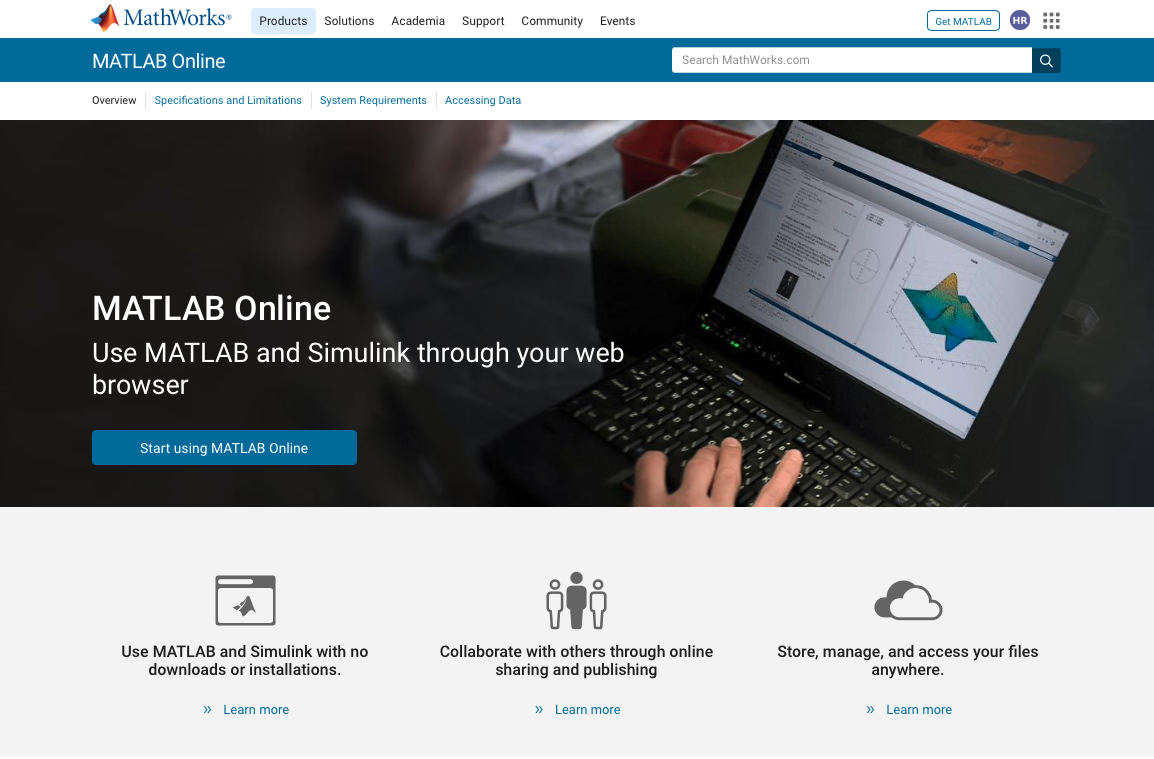
\includegraphics[width=0.9\textwidth]{matlab_online}
\end{center}
\url{https://matlab.mathworks.com}
\end{frame}



\begin{frame}{MATLAB Graphical Interface}
\begin{columns}
\begin{column}[T]{0.35\textwidth}
\begin{itemize}
	\item Command window
	\item Workspace
	\item Current folder
	\item Command history
	\item Editor
	\end{itemize}
\end{column}
\begin{column}[T]{0.75\textwidth}
	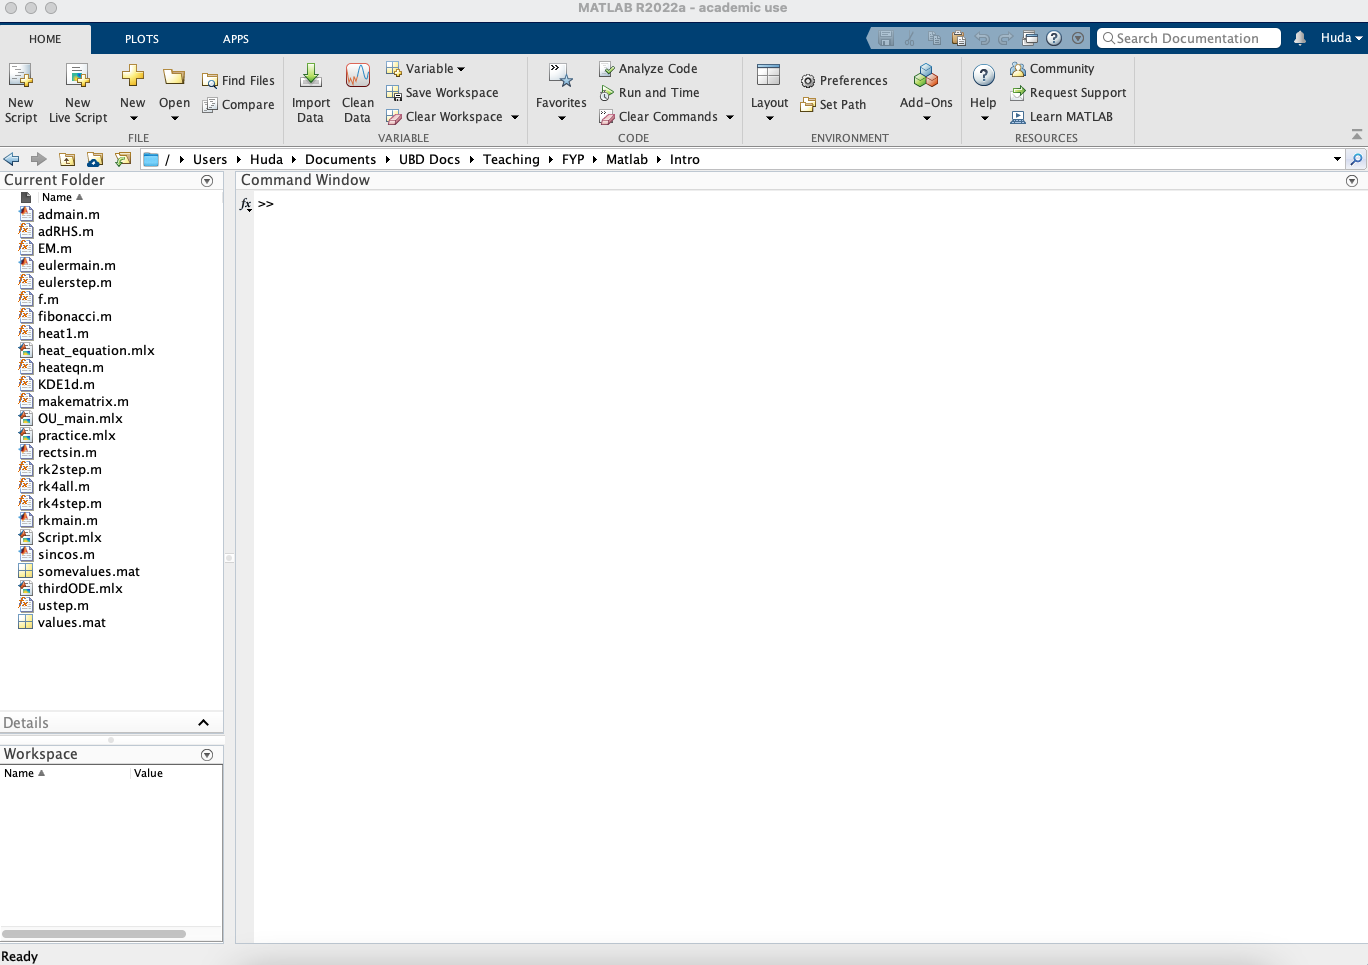
\includegraphics[width=0.9\textwidth]{initial_matlab}
\end{column}
\end{columns}




\end{frame}

